\documentclass[../ASSD_TP2.tex]{subfiles}
\begin{document}
\section*{Síntesis basada en muestras}
\subsection*{Introducción}
El objetivo de la síntesis basada en muestras es poder conseguir distintas notas y duración de un instrumento, a partir de una muestra. Para lograrlo basta con resolver uno de dos problemas:
\begin{itemize}
\item Alterar la frecuencia fundamental si modificar la duración
\item Modificar la duración sin alterar la frecuencia fundamental
\end{itemize}

Solucionado uno de los previamente mencionado vasta resamplear la se\~nal con una frecuencia distintas. Por ejemplo si se resamplea a una frecuencia de sampleo del doble, se alteraría la frecuencia fundamental pero también la duración, por ende bastaría con alargarlo en el tiempo sin alterar la frecuencia.
\subsection*{TME(Time Scale Modification)}
Tal como su nombre lo indica, refiere  algoritmos con la capacidad de alterar la longitud temporal de una muestra. El algoritmo mas sencillo capaz de lograrlo es el resampling:

\begin{lstlisting}
def resampling(x,Fs,scale):
	y=interpolate(x)
	y=sample(y,scale*Fs)
	return y
\end{lstlisting}
A pesar de su sencillez el problema fundamental de este algoritmos es que altera las frecuencias de las muestras. Por ende para evitar este problema se requieren algoritmos mas complejos.
\subsubsection*{OLA(Overlap and add)}
El principio de funcionamiento del algoritmo, es tomar segmentos del fragmento original y superponerlos hasta obtener la longitud deseada.
\begin{figure}


  \centering
   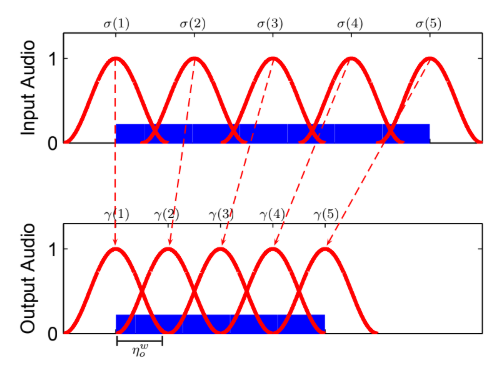
\includegraphics[width=0.9\textwidth]{figures/ola.png}
  \caption{Ejemplo del funcionamiento del algoritmo, imagen obtenia de Driedger Jonathan TSM Master Thesis}
\end{figure}
\subsubsection*{WSOLA}

\subsection*{PSOLA}


\end{document}
